\documentclass[11pt]{standalone}

\usepackage{lmodern}	% font definition
\usepackage{amsmath}	% math fonts
\usepackage{amsthm}
\usepackage{amsfonts}
\usepackage{pgfplots}

\usepackage{pgfplots}
\usepackage{xcolor}
\usetikzlibrary{positioning,bayesnet}
\definecolor{brinkpink}{rgb}{0.98, 0.38, 0.5}
\definecolor{aogreen}{rgb}{0.0, 0.5, 0.0}
\usepackage{tikz}
\usetikzlibrary{decorations.pathmorphing} % noisy shapes
\usetikzlibrary{fit}					% fitting shapes to coordinates
\usetikzlibrary{backgrounds}	% drawing the background after the foreground
\pgfplotsset{compat=newest}% <-- moves axis labels near ticklabels (respects tick label widths)

\begin{document}
  \pgfplotsset{every tick label/.append style={font=\normalsize}}
  \pgfplotsset{every axis label/.append style={font=\normalsize}}
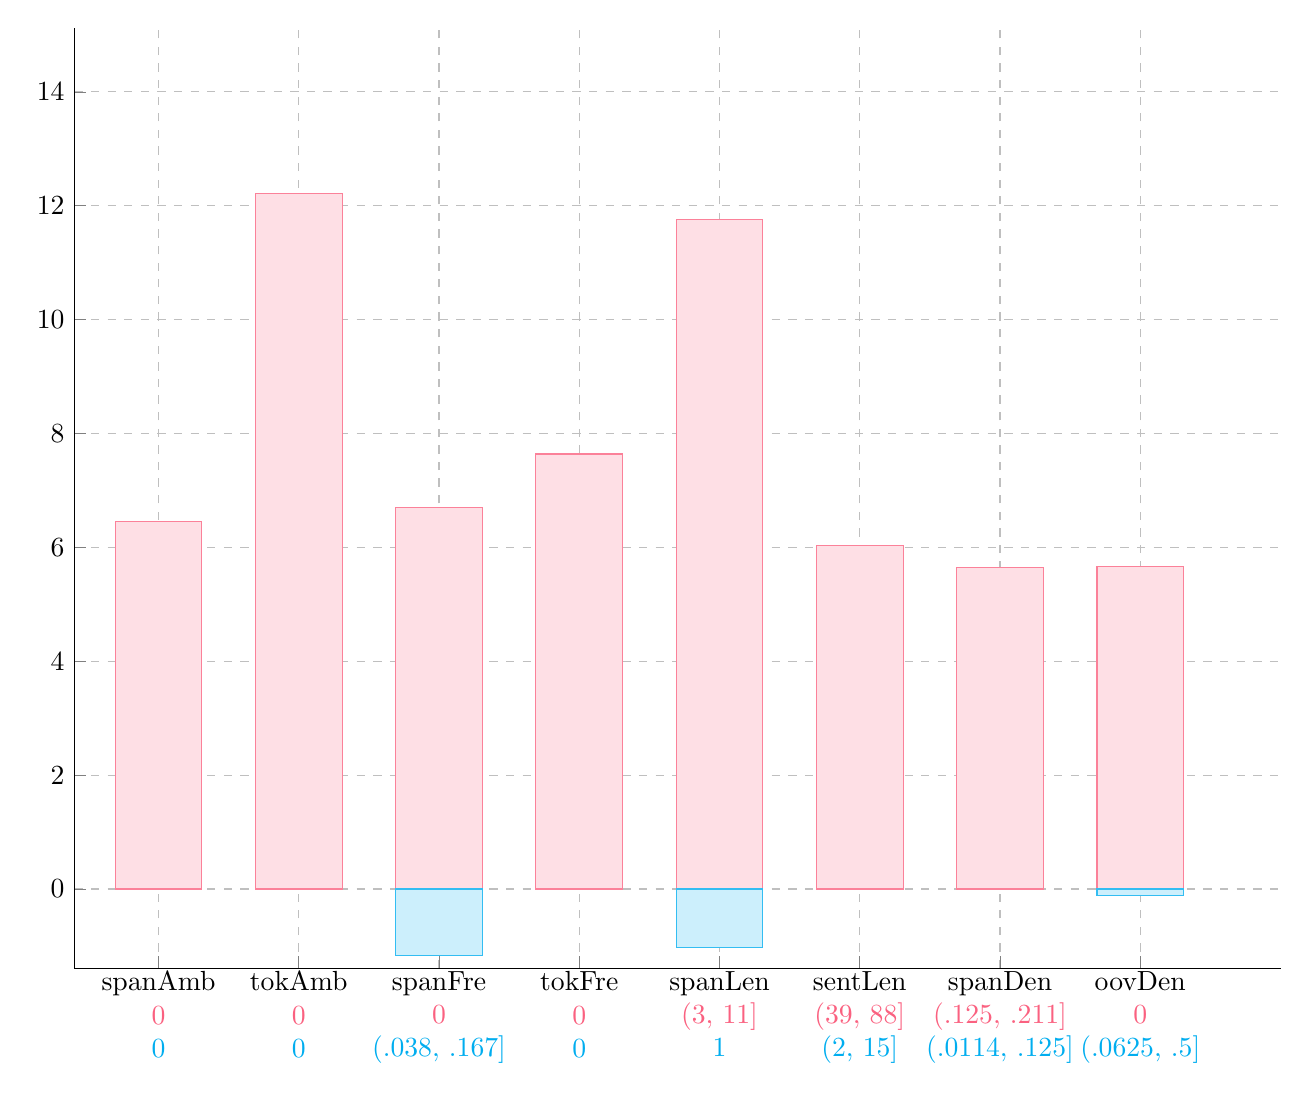
\begin{tikzpicture}
  \centering
  \begin{axis}[%ybar=1.0pt,
    ybar stacked,
    height=13.52cm,
    %width=16.9cm, % 12->9,  9->6.93,  8-> 6
    width=16.9cm, % 12->9,  9->6.93,  8-> 6
    bar width=1.1cm,
    xmin=0.4,
    xmax=9,
    ymin=-1.392,
    ymax=12.963333333333335,
    enlarge y limits={upper,value=0.15},
    axis lines*=left,
    legend style={at={(0.5,-0.25)},anchor=north,legend columns=-1,
    /tikz/every even column/.append style={column sep=0.2cm}},
    %xticklabels={\textcolor{brinkpink}{S}-\textcolor{aogreen}{L},\textcolor{brinkpink}{M}-\textcolor{aogreen}{S},\textcolor{brinkpink}{L}-\textcolor{aogreen}{M},\textcolor{brinkpink}{S}-\textcolor{aogreen}{S},\textcolor{brinkpink}{M}-\textcolor{aogreen}{M},\textcolor{brinkpink}{L}-\textcolor{aogreen}{L},\textcolor{brinkpink}{S}-\textcolor{aogreen}{S},\textcolor{brinkpink}{M}-\textcolor{aogreen}{M}},
    xticklabels={spanAmb \\ \textcolor{brinkpink}{0} \\ \textcolor{cyan}{0}, tokAmb \\ \textcolor{brinkpink}{0} \\ \textcolor{cyan}{0}, spanFre \\ \textcolor{brinkpink}{0} \\ \textcolor{cyan}{(.038, .167]}, tokFre \\ \textcolor{brinkpink}{0} \\ \textcolor{cyan}{0}, spanLen \\ \textcolor{brinkpink}{(3, 11]} \\ \textcolor{cyan}{1}, sentLen \\ \textcolor{brinkpink}{(39, 88]} \\ \textcolor{cyan}{(2, 15]}, spanDen \\ \textcolor{brinkpink}{(.125, .211]} \\ \textcolor{cyan}{(.0114, .125]}, oovDen \\ \textcolor{brinkpink}{0} \\ \textcolor{cyan}{(.0625, .5]}},
    xtick=data,
    xmajorgrids=true,
    ymajorgrids=true,
    zmajorgrids=true,
    grid style=dashed,
    xticklabel style={
        inner sep=1pt,
	align=center,
        %rotate=90,
        %anchor=near xticklabel,
    },
    ]
    %\addplot [draw=aogreen!80,fill=aogreen!20] table[x=id,y=y]{
    \addplot [draw=cyan!80,fill=cyan!20] table[x=id,y=y]{
    id  y
    	1	0.0
	2	0.0
	3	-1.16
	4	0.0
	5	-1.02
	6	0.0
	7	0.0
	8	-0.11
    };
    \addplot [draw=brinkpink!80,fill=brinkpink!20] table[x=id,y=y]{
    id  y
    	1	6.45
	2	12.22
	3	6.7
	4	7.64
	5	11.75
	6	6.04
	7	5.64
	8	5.67
    };
  \end{axis}
\end{tikzpicture}

\end{document}

